\documentclass[15pt]{article}
\usepackage[utf8]{inputenc}
%\renewcommand{\baselinestretch}{1.3}
\usepackage[czech]{babel}

% není úplně potřeba, takže pak odstranit
\usepackage{xcolor}
\usepackage{comment}

\usepackage{amsmath}
\usepackage{amssymb}
\usepackage{algorithm}
\usepackage{algorithmicx}
\usepackage{gensymb}

\usepackage[margin=1in]{geometry}
\usepackage{setspace}
\usepackage{parskip}
\setlength{\parindent}{20pt}

\usepackage{fancyhdr}
\pagestyle{fancy}
\rhead{Point Location Problem}
\lhead{Algoritmy počítačové kartografie}

\usepackage{graphicx}
\graphicspath{ {./images/} } 

\begin{document} 

% TITULNÍ STRÁNKA
\begin{titlepage}
    %\begin{center}
        \centering
        {\large Přírodovědecká fakulta
        
        Univerzita Karlova\par}
        \vspace{1cm}
        
\includegraphics[scale=0.4]{images/logo.png}\\
        \vspace{2cm}
        {\large Algoritmy počítačové kartografie}\\
        {\huge Úkol č. 1: Point Location Problem \par}
        \vspace{0.5cm}
        {\large Vanda Hlaváčková a Petra Krsková \par}
        \vspace{2cm}
        1.N-GKDPZ
    
        Praha 2023
        \vspace{3cm}
    %\end{center}
\end{titlepage}

\begin{spacing}{1.5}

% ZADÁNÍ 
\section*{Zadání}
\subsection*{\textbf{Úloha č. 1: Geometrické vyhledávaní bodu}}
\noindent\textit{Vstup: Souvislá polygonová mapa n polygonů \{$P_1, ..., P_n$\}, analyzovaný bod q.}

\noindent\textit{Výstup: $P_i, q \in P_i$.}

\noindent Nad polygonovou mapou implementujete Ray Crossing Algorithm pro geometrické vyhledávání incidujícího polygonu obsahujícího zadaný bod $q$.

\noindent Nalezený polygon graficky zvýrazněte vhodným způsobem (např. vyplněním, šrafováním, blikáním). Grafické rozhraní vytvořte s využitím frameworku QT.

\noindent Pro generování nekonvexních polygonů můžete navrhnout vlastní algoritmus či použít existující geografická data (např. mapa evropských států).

\noindent Polygony budou načítány z textového souboru ve Vámi zvoleném formátu. Pro datovou reprezentaci jednotlivých polygonů použijte špagetový model.

\vspace{1cm}
\subsection*{\textbf{Hodnocení:}}

\begin{center}
\begin{tabular}{|l|l|}
\hline
\textbf{Krok}                                                                                  & \textbf{hodnocení} \\ [0.5ex]  \hline\hline
Detekce polohy bodu rozšiřující stavy uvnitř, vně polygonu.                                    &  10 b.              \\ \hline
\textit{Analýza polohy bodu (uvnitř/vně) metodou Winding Number Algorithm.}                    & \textit{+10 b.}    \\ \hline
\textit{Ošetření singulárního případu u Winding Number Algorithm: bod leží na hraně polygonu.} & \textit{+ 5 b.}    \\ \hline
\textit{Ošetření singulárního případu u Ray Crossing Algorithm: bod leží na hraně polygonu.}   & \textit{+ 5 b.}    \\ \hline
\textit{Ošetření singulárního případu obou algoritmů: bod je totožný s vrcholem jednoho či více polygonů.} & \textit{+ 2 b.} \\ \hline
\textit{Zvýraznění všech polygonů pro oba výše uvedené singulární případy.}                    & \textit{+ 3 b.}    \\ \hline
\end{tabular}
\end{center}

% POPIS A ROZBOR PROBLÉMU
\newpage
\section*{Popis a rozbor problému}
\subsection*{Point Location Problem}
\textit{Point Location Problem} se řadí k nejdůležitějším a nejčastěji řešeným problémům počítačových aplikací využívajících geometrické struktury. Mezi takové aplikace se například řadí robotika, databáze nebo geoinformační systémy. Problém se snaží odpovědět na otázku, jestli se definovaný bod nalézá uvnitř, mimo nebo zda leží na hraně/vrcholu mnohoúhelníku tvořeného množinou m bodů (Guaily, Karim 2020).  

Tento pro člověka triviální úkol, který je schopen vyřešit pohledem během několika sekund, je z hlediska automatizace poměrně obtížný. K jeho řešení může být aplikováno několik algoritmů.  Řada z nich naráží na problém vhodného ošetření singularit, a často tak tyto algoritmy vyžadují specifickou reprezentaci dat a jejich předzpracovatelskou úpravu. Mimo ošetření singularit naráží řada algoritmů i na velkou časovou náročnost nebo na nedostatek paměti pro zpracování příslušných dat (Huang and Shih 1997; Kumar, Bangi 2018).  

Obecně lze polygony rozdělit do dvou kategorií, a to na konvexní a nekonvexní. U konvexních nepřesahují úhly tvořené spojením vrcholů 180°. Naopak u nekonvexního mnohoúhelníku je alespoň jeden úhel, který tuto hodnotu přesahuje. Vzhledem k častějšímu výskytu nekonvexních mnohoúhelníků se tato práce dále věnuje dvěma pro tyto polygony často používaným algoritmům, a to $Winding$ $Number$ a $Ray$ $Crossing$ (Martín, Zapata 2012).

% WINDING NUMBER
\subsection*{Winding Number Method}
Algoritmus Winding Number představuje sumu $\Omega$ všech úhlů $\omega_1$, které svírá pozorovaný bod $q$ s vrcholy $P$ daného mnohoúhelníku. 
\begin{equation*}
\Omega (q,P)= \begin{cases}
    1, q  \in P \\
    0, q  \notin P\\
\end{cases}
\end{equation*}
 
 \noindent Pro výpočet polohy bodu $q$ vůči přímce  $p \approx \overleftrightarrow{P_iP_{i+1}}$, je nutné nejprve vypočítat směrový vektor přímky $q$ a vektor $v$, který je určen bodem $q$ a $p_i$.
 \begin{align}
    \nonumber&\vec{p}=(x_{i+1}-x_i,y_{i+1}-y_i)\\
    \nonumber&\vec{v}=(x_q-x_i,y_q-y_i)
\end{align}
Následně lze tyto vektory přepsat jako matici, kdy hodnota determinantu určuje, ve které polorovině se bod $q$ nachází. Jednotlivé poloroviny od sebe odděluje právě přímka $p$. 

\begin{equation*}
d=\begin{vmatrix} q_x & q_y \\ v_x & v_y  \end{vmatrix}=
\begin{cases}
    >0, \quad q  \in \sigma_l \\
    =0, \quad q  \in p\\
    <0, \quad q \in \sigma_r
\end{cases}
\end{equation*}

\noindent V případě, že se bod $q$ nachází v levé polorovině ($\sigma_l$), je úhel orientován ve směru hodinových ručiček. U pravé poloviny ($\sigma_r$) je to naopak, výsledná hodnota $\Omega$ vychází záporně. Výsledek je poté uváděn jako počet oběhů, tedy v násobcích $2 \pi$ (Martín, Zapata 2012).  

Výhodou $Winding Number Algoritmu$ je jeho lepší ošetření v singulárních případech, oproti paprskovému algoritmu. Zároveň je však pomalejší a problém nastává, když je poloha hledaného bodu totožná s polohou jednoho z bodů tvořící mnohoúhelník (Martín, Zapata 2012). 

% pseudokód winding number
\subsubsection*{Pseudokód metody Winding Number}
\begin{algorithm}
    \caption {\textit{Winding Number}}
    \begin{algorithmic}[1]
        \State $\varOmega$ = 0, tolerance $\epsilon$
        \State zkontroluj, zda bod $q$ není totožný s vrcholem
        \State pro všechny hrany (tvořena body $p_i$ a $p_{i+1}$):
        \State \indent urči polohu bodu $q$ vůči hraně
        
        \State \indent vypočti úhel $\omega$ mezi $q$ a $p_i$ a $p_{i+1}$
        \State \indent \textbf{pokud} $q \in \sigma_l$:
        \State \indent  \indent $\varOmega + \omega$
        \State \indent \textbf{pokud} $q \in \sigma_r$:
        \State \indent \indent $\varOmega - \omega$
        \State \indent {\textbf{jinak pokud}} $q$ leží mezi $p_i$ a $p_{i+1}$
        \State \indent \indent $q \in \partial P$
        
        \State \textbf{pokud} $|\varOmega| - 2\pi < tolerance$:
        \State \indent $q \in P$
        \State \textbf{jinak} $q \notin P$
    \end{algorithmic}
\end{algorithm}

% RAY CROSSING METHOD
\subsection*{Ray Crossing Method}
Algoritmus $Ray$ $Crossing$ je představován přímkou $r$, která je vedena v libovolném směru zkoumaným bodem $q$. Počet hran, které přímka $r$ protíná, je značen písmenem $k$. V případě, že je tato hodnota po vydělení dvěma rovna nula, leží zkoumaný bod uvnitř polygonu. Aby bod ležel mimo polygon, hodnota $k$ po vydělení dvěma by musela být nulová. 

\begin{equation*}
k\%2=\begin{cases}
    0, \quad q  \notin P\\
    1, \quad q  \in P\\
\end{cases}
\end{equation*}

Jak již bylo výše zmíněno, přímku $r$ lze vést pod libovolným úhlem. Problém nastává u singularit, tedy v případě, že přímka prochází vrcholem mnohoúhelníku $P$ nebo je totožná s jeho hranou. Možným řešením je variace metody $Ray$ $Crossing$ s redukcí ke $q$. Při ní dochází k přepočítání vrcholů mnohoúhelníku, a to na základě posunutí počátku souřadnicového systému do bodu $q$. Tato metoda ale neumí rozpoznat, zda se zkoumaný bod $q$ nachází na hraně mnohoúhelníku $P$. Pro detekci tohoto stavu je nutné přidat další polopřímku. $r_1$ má levostrannou orientaci a $r_2$ pravostrannou. 

V případě, že se počet průsečíků $k_l$ a $k_r$ s polopřímkami $r_1$ a $r_2$ nerovná, bod $q$ se nachází na hraně polygonu $P$. Ověření stejnolehlosti bodu $q$ s vrcholem polygonu je zjišťováno porovnáváním souřadnic bodu $q$ s každým vrcholem vstupních dat. Pokud souřadnice vrcholu i bodu $q$ souhlasí, nachází se bod $q$ na vrcholu daného mnohoúhelníku (Bayer 2023). V neposlední řadě stejně jako u verze bez redukce k bodu $q$ platí, že bod se nachází uvnitř polygonu tehdy, když je počet průsečíků $k_r$ s polopřímkou $r_1$ lichý. 


% pseudokód ray crossing 
\subsubsection*{Pseudokód metody Ray Crossing}
\begin{algorithm}
    \caption {\textit{Ray Crossing}}
    \begin{algorithmic}[1]
        \State inicializuj $k_r$ a $k_l$ na 0 a počet vrcholů $n$
        \State pro všechny vrcholy:
        \State \indent vypočti nové (redukované) souřadnice $x_{ir}, y_{ir}$, $x_{i+1r}, y_{i+1r}$\\
        
        \State \indent \textbf{pokud} $x_{ir} = 0$ a $y_{ir} = 0$
        \State \indent \indent $q$ je totožný s vrcholem

        \State \indent \textbf{pokud} $y_{i+1r} - y_{ir}$ = 0 (horizontální hrana)
        \State \indent \indent jdi na další uzel\\

        \State \indent vypočti $x$ souřadnice průsečíku $x_m$ 
        % levá přímka r_2
        \State \indent \textbf{pokud} $(y_i < 0) \neq (y_{i+1}<0)$ (levostranný paprsek)
        \State \indent \indent \textbf{pokud} $x_m<0$:
        \State \indent \indent \indent zvyš počet průsečíků $k_l$

        % pravá přímka r_1
        \State \indent \textbf{pokud} $(y_i>0) \neq (y_{i+1}>0)$ (pravostranný paprsek) 
        \State \indent \indent \textbf{pokud} $x_m>0$:
        \State \indent \indent \indent  zvyš počet průsečíků $k_r$\\
        
        \State \textbf{pokud} $(k_l\%2) \neq (k_r\%2)$
        \State \indent $q \in \partial P$
        \State \textbf{pokud} $k_r\%2 = 1$
        \State  \indent $q \in P$
        \State \textbf{jinak} $p \notin P$
    \end{algorithmic}
\end{algorithm}

% APLIKACE
\subsection*{Aplikace}
Aplikace pro analýzu polohy bodu vzhledem k polygonu byla vytvořena v prostředí $Qt Creator$ a jsou v ní implementovány oba výše popsané algoritmy – $Winding Number$ i $Ray Crossing$.

Po spuštění aplikace přes soubor $mainform.py$ je otevřeno okno, jehož většinu tvoří prázdná plocha pro vykreslení polygonů. V horní části se pak nachází menu s jednotlivými funkcemi. V záložce $File$  je možné pomocí funkce $Open$ vyvolat dialogové okno a vybrat vstupní data ve formátu $.shp$, která jsou následně vykreslena (viz obr. 1). Možnost $Exit$ pak slouží k zavření aplikace. 

\begin{figure}
    \centering
    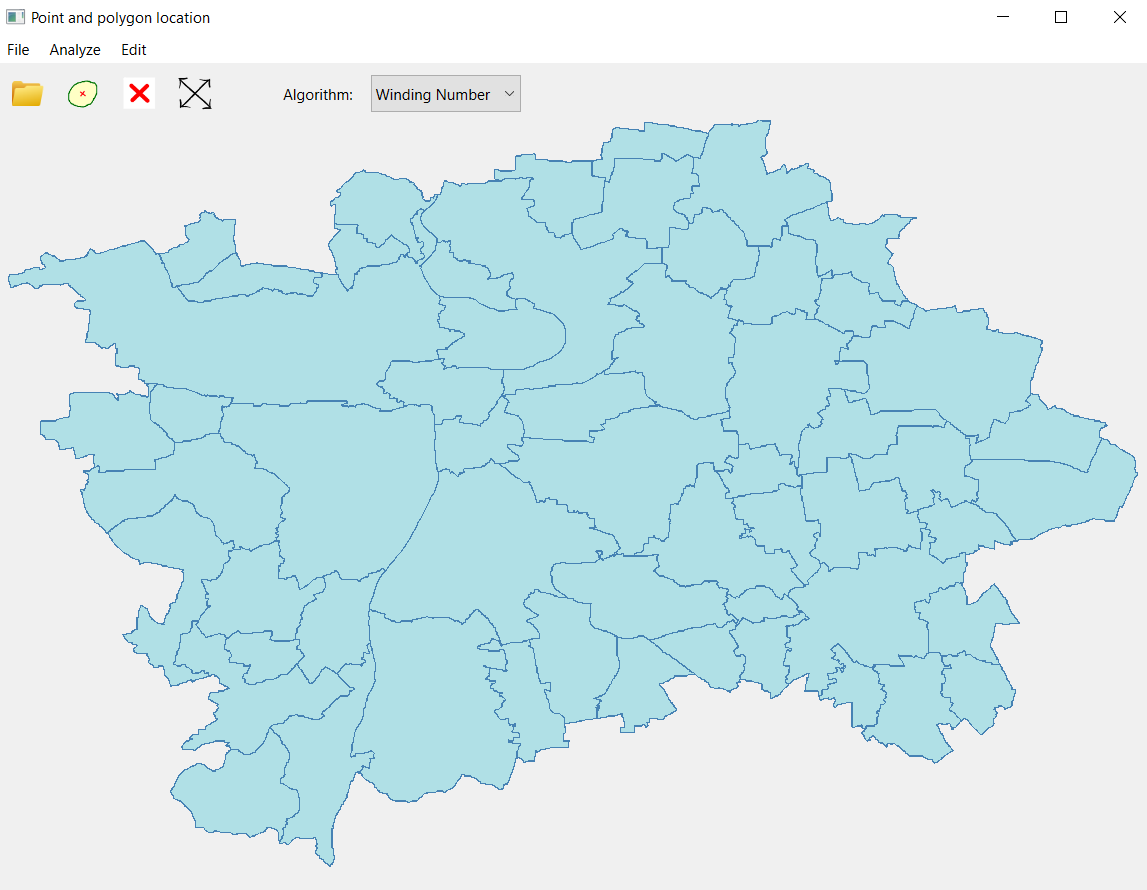
\includegraphics[scale=0.55]{images/aplikace.png}
    \textit{\caption{ukázka aplikace}}
\end{figure}

Kliknutím do okna je vykreslen bod, jehož poloha vůči polygonu je zanalyzována po výběru funkce $Point In Polygon$ v záložce $Analyze$. Následně je zvýrazněn polygon, ve kterém bod leží (viz obr. 2), v případě umístění bodu na hranu či vrchol, jsou vykresleny všechny polygony, kterým daná hrana nebo vrchol náleží (viz obr. 3). V pravé části menu je pomocí rozbalovacího seznamu možné vybrat, který algoritmus má být pro analýzu využit. Při zvětšení okna aplikace je možné přizpůsobit zobrazení dat funkcí $Fit To Display$ v záložce $Edit$. Možností $Clear$ jsou pak vymazány nahrané polygony.

Popsané funkce je možné vyvolat i pomocí ikon umístěnými pod záložkami menu, v pořadí zleva se jedná o funkce $Insert file$, $Analyze point and polygon position$, $Clear$ a $Fit to display$. Ikony odpovídají jednotlivým funkcím v záložkách menu a po umístění kurzoru myši na ikonu je vypsán i název odpovídající funkce.

\begin{figure}
    \centering
    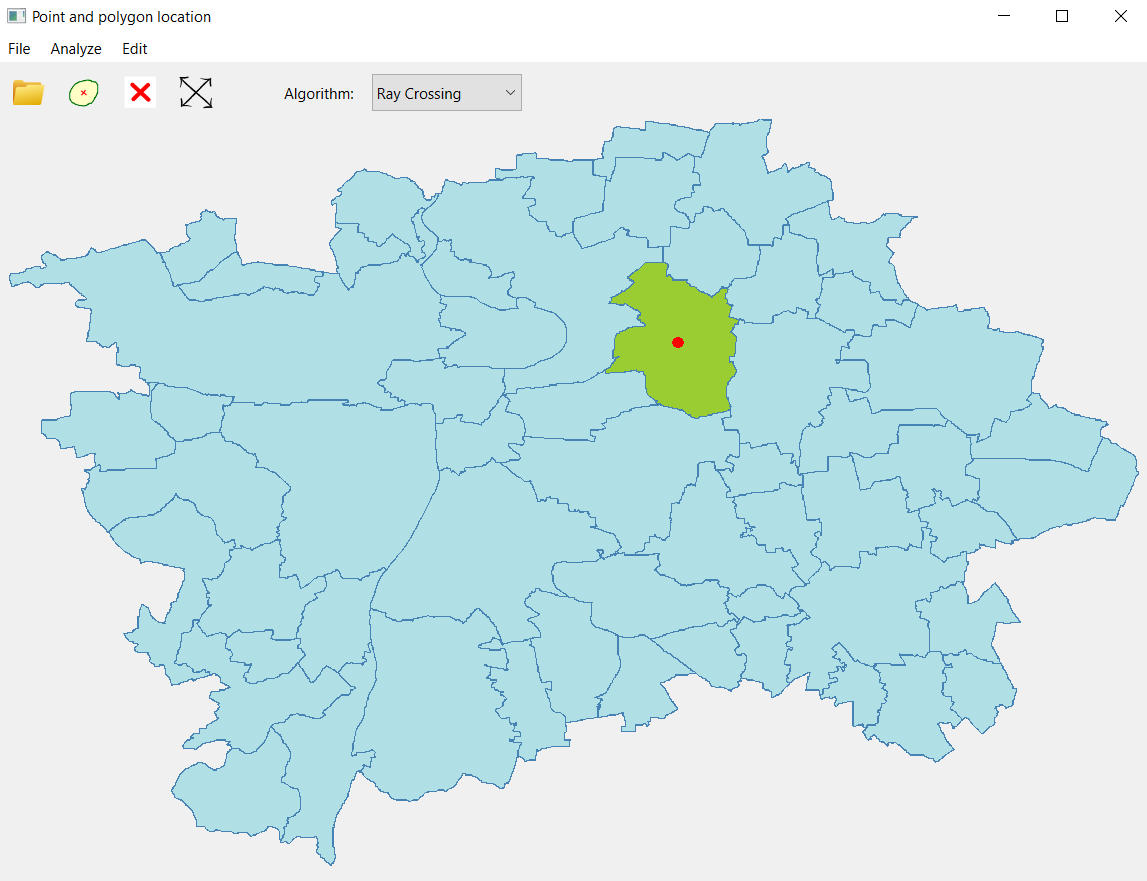
\includegraphics[scale=0.55]{images/uvnitr_polygonu.png}
    \textit{\caption{bod leží uvnitř polygonu}}
\end{figure}

\begin{figure}
    \centering
    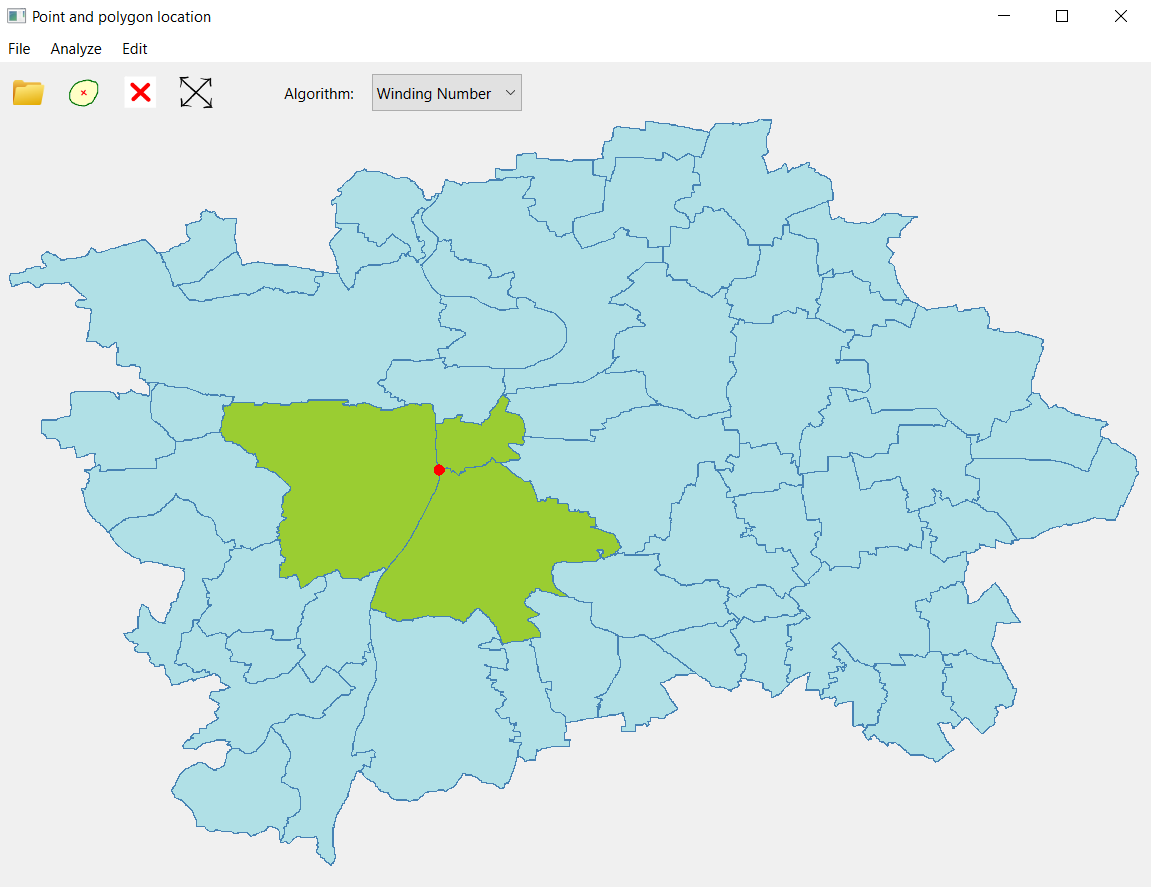
\includegraphics[scale=0.55]{images/hrana_vrchol.png}
    \textit{\caption{bod je totožný s vrcholem více polygonů}}
\end{figure}

% DOKUMENTACE
\newpage
\subsection*{Dokumentace programu}
Program byl vytvořen v prostředí PyCharm v programovacím jazyce Python s využitím $Qt Creator$ a modulu $pyshp$, který umožňuje práci se shapefily. Program se skládá ze souborů $mainform.py$, $draw.py$ a $algorithms.py$, které obsahují názvům odpovídající třídy. Ve složce $icons$ se pak nachází pět obrázkových souborů využitých pro ikony jednotlivých funkcí.

\subsubsection*{třída MainForm:}
Tato třída slouží pro konfiguraci uživatelského rozhraní aplikace a jeho propojení na metody definované v ostatních třídách. Třída obsahuje šest metod.
Metody $setupUi$ a $retranslateUi$ byly vytvořeny automaticky na základě vytvořeného prostředí v $Qt Creator$. V první z nich jsou na řádkách 113–121 napojeny jednotlivé položky menu a tlačítka na připravené metody.

\noindent Metoda $openFile$ ukládá do proměnných $width$ a $height$ aktuální šířku a výšku okna pro vykreslování polygonů. Následně volá metody $loadData$ a $rescaleData$ třídy $Draw$, čímž dochází k načtení vstupních dat a jejich vykreslení.

\noindent Metoda $analyze$ slouží pro analýzu polohy bodu vůči polygonu. Metodami $getPoint$ a $getPolygons$ z třídy $Draw$ získá aktuální polohu bodu a seznam vykreslených polygonů. Dále jsou postupně procházeny všechny polygony a pomocí aktuálního indexu rozbalovacího seznamu (comboBox) je kontrolováno, který algoritmus pro analýzu je vybrán a na jeho základě je volána metoda $windingNumber$ nebo $rayCrossing$ třídy $Algorithms$. V obou případech je výsledek analýzy předán funkci $setResult$ třídy $Draw$. Na závěr je vyvolána metoda na překreslení okna, aby došlo ke zvýraznění polygonu obsahující bod.

\noindent Metoda $clearCanvas$ slouží k vymazání nahraných polygonů a volá metodu $clearPol$ třídy $Draw$. 

\noindent Poslední metoda $fitToDisplay$ slouží k překreslení polygonů při změně velikosti okna tak, aby jí odpovídaly a vyplňovaly celou plochu. Do proměnných $width$ a $height$ načítá aktuální šířku a výšku okna pro vykreslování polygonů a poté volá metodu $rescaleData$ třídy $Draw$ a vyvolává funkci pro překreslení okna

\subsubsection*{třída Draw:}
Tato metoda zajišťuje grafické rozhraní aplikace a obsahuje devět metod.

Inicializační metoda má dva poziční argumenty a dochází v ní k inicializaci šesti proměnných. Vykreslovaný bod  $q$ je typu $QPointF$ a počáteční souřadnice jsou mu nastaveny tak, aby se vykreslovat mimo okno. Dále dochází k inicializaci seznamu polygonů ($polygons$) a seznamu, do kterého se při každém spuštění analýzi ukládá výsledek pro jednotlivé polygony ($pol_res$). Proměnná $features$ sloužící pro ukládání objektů z načteného shapefilu je inicializována jako $None$. Dále je inicializován seznam $min_max$ pro ukládání minimálních a maximálních souřadnic polygonů a proměnná $no_data$.

\noindent Metoda $loadData$ slouží k načtení vstupních dat. Nejprve dochází k vyvolání dialogového okna, ze kterého je získána cesta k souboru se vstupními daty. Pokud je okna zavřeno bez vybrání souboru, dochází k aktualizaci proměnné $no_data$ na hodnotu $True$ a ukončení metody. V opačném případě jsou funkcemi modulu $pyshp$ získány jednotlivé objekty ze vstupního souboru. Na závěr dochází k projdutí všech polygonů a jejich bodů a získání minimální a maximální X a Y souřadnice.

\noindent Metoda $rescaleData$ slouží k úpravě souřadnic bodů jednotlivých polygonů, aby je bylo možné vykreslit v okně aplikace. Na vstupu má argumenty $width$ a $height$, které odpovídají aktuální šířce a výšce okna pro vykreslení polygonů. Pokud je proměnná $no_data$ nastavena na hodnotu $True$, dojde k vytvoření jednoho polygonu, který se nachází mimo vykreslovací okno, čímž je zabráněno pádu aplikacepři nezvolení cesty k souboru se vstupními daty. 

V opačném případě je inicializován seznam polygonů podle počtu objektů proměnné $features$. Tyto objekty jsou následně procházeny a všem jejich bodům jsou na základě minimálních a maximálních souřadnic a velikosti vykreslovacího okna přepočítány souřadnice. Po úpravě souřadnic dochází k vytvoření bodu typu $QPointF$ a jeho přidání do příslušného polygonu.

\noindent Metoda $mousePressEvent$ má vstupní argument odpovídající kliknutí myši. Odečítá aktuální souřadnice kurzoru myši a předává je bodu $q$. Na závěr dochází k vyvolání metoda pro překreslení okna, aby došlo k vykreslení nové pozice bodu.
\noindent Metoda $paintEvent$ má na vstupu argument $QPaintEvent$. Tato metoda slouží k vykreslení polygonů a bodu. Pomocí $for$ cyklu jsou procházeny všechny polygony a je jim nastavena jednotná barva, s jakou se mají vykreslit. Zároveň dochází ke kontrole hodnoty daného polygonu v seznamu výsledků, a pokud odpovídá 1 (bod leží v polygonu) nebo -1 (bod leží na hraně nebo vrcholu polygonu), dojde k nastavení jiné barvy pro daný polygon. Následně je každý polygon vykreslen a seznam výsledků je vymazán pro další analýzu. Na závěr dochází k nastavení barvy a velikosti bodu a k jeho vykreslení.

\noindent Metoda $setResult$ má jako vstupní argument výsledek analýzy, který připojuje na konec seznamu $pol_res$.

\noindent Metoda $clearPol$ slouží k vymazání vykreslených polygonů a bodu. Seznam s polygony je tak vymazán a bodu jsou nastaveny souřadnice mimo okno. Na závěr je vyvolána metoda pro překreslení okna.

\noindent Metody $getPoint$ a $getPolygon$ předávají vytvořený bod a seznam polygonů.

\subsubsection*{třída Algorithms:}
Tato třída v sobě implementuje algoritmy pro analýzu polohy bodu a polygonu.

\noindent Metoda $getPointAndEdgePosition$ má jako vstupní argumenty vykreslený bod $q$ a body $p1$ a $p2$ tvořící hranu polygonu a slouží k určení polohy analyzovaného bodu a hrany polygonu. Nejprve dochází k výpočtu vektoru mezi bodem $q$ a počátečním vektorem hrany a vektoru mezi body hrany. Následně dochází k výpočtu determinantu a podle jeho výsledku je metodou vrácena hodnota 1, pokud bod leží v levé polorovině od hrany, hodnota 0, pokud bod leží v pravé polorovině, a hodnota -1 v ostatních případech, tedy kdy bod leží na hraně.

\noindent Metoda $getAngle$ má jako vstupní parametry analyzovaný bod $q$ a body $p1$ a $p2$ tvořící hranu polygonu a slouží k určení úhlu mezi bodem a koncovými body hrany. Nejprve jsou spočítány vektory mezi bodem $q$ a krajními body hrany. Následně je vypočítán jejich skalární součin a norma obou vektorů. Pokud je jedna z norem vektorů nulová, bod $q$ je shodný s bodem hrany a metoda vrátí hodnotu 0. Pro správnou funkčnost funkce $acos$ je zkontrolováno, zda není vypočítaná hodnota cosinu větší než 1 nebo menší než -1 a případně je na tuto hodnotu zaokrouhlena a metoda vrací hodnotu úhlu. Jinak dochází k výpočtu úhlu a navrácení jeho hodnoty.

\noindent Metoda $windingNumber$ má jako vstupní argumenty analyzovaný bod $q$ a polygon, vůči kterému se analyzuje poloha bodu a implementuje metodu $Winding Number$. Nejprve dochází k inicializaci proměnné pro součet úhlů a tolerance $epsilon$ a následně dochází k procházení všech vrcholů polygonu. Pokud se obě souřadnice vrcholu rovnají souřadnicím bodu, znamená to, že bod leží na vrcholu polygonu a metoda vrátí hodnotu -1. Jinak je pomocí dvou předchozích metod určena poloha bodu vůči hraně polygonu a úhel. Pokud bod leží v levé polorovině, vypočítaný úhel je připočten k sumě úhlů. Pokud se bod nachází v pravé polorovině, je úhel od této sumy odečten. V ostatních případech bod leží na přímce, která prochází hranou. Pomocí vektorů mezi bodem a krajními body hrany dochází k ověření, zda bod leží mezi nimi a tím pádem na hraně a při splnění této podmínky metoda vrátí hodnotu -1. Jinak je zkontrolováno, zda je rozdíl sumy úhlů od $2\pi$ menší než definovaná tolerance a pokud ano, bod leží v polygonu a metoda vrátí hodnotu 1. V opačném případě bod leží mimo polygon a metoda vrátí hodnotu 0.

\noindent Metoda $rayCrossing$ má jako vstupní argumenty analyzovaný bod $q$ a polygon, vůči kterému se analyzuje poloha bodu a implementuje metodu $Ray Crossing$ s redukcí souřadnic k bodu $q$ a dvěma paprsky pro detekci bodu na hraně. Nejprve jsou inicializovány proměnné udržující počet levých a pravých průsečíků a počet vrcholů polygonu. Dále jsou procházeny všechny vrcholy polygonu a pro vrcholy tvořící hranu jsou redukovány souřadnice k bodu $q$. Pokud jsou redukované souřadnice prvního bodu nulové, znamená to, že bod leží na tomto vrcholu a metoda vrátí hodnotu -1. V případě nulového rozdílu mezi ypsilonovými souřadnicemi vrcholů se jedná o horizontální hranu a dochází ke skoku na další hranu polygonu. Následně dochází ke kontrole, zda se jedná o levostranný či pravostranný paprsek a k výpočtu průsečíku. Pokud průsečík splňuje zadanou podmínku, je inkrementována příslušná proměnná. V případě, že se počet levostranných a pravostranných průsečíků nerovná, bod leží na hraně a metoda vrátí hodnotu -1. Pokud je počet pravostranných průsečíků lichý, bod leží uvnitř polygonu a dojde k navrácení hodnoty 1. V ostatních případech bod leží mimo polygon a metoda vrátí hodnotu 0.

% ZÁVĚR
\subsection*{Závěr}
V rámci této úlohy byla vytvořena aplikace která na základě uživatelem zvoleného algoritmu ($Winding$ $Number$ nebo $Ray$ $Crossing$) analyzuje polohu zvoleného bodu vůči daným polygonům včetně ošetření singularit, a sice, že je bod totožný s vrcholem nebo hranou polygonu. 

Možným zlepšením aplikace by bylo jiné ošetření zavření dialogového okna při načítání vstupních dat bez vybrání souboru. Momentálním řešením je tvorba skrytého polygonu mimo plochu pro vykreslení polygonů. Při prvním načítání vstupních dat nebo po vyčištění plochy funkcí $Clear$ se nic nestane a plocha zůstane prázdná, při zavření dialogového okna v případě, že jsou v aplikaci vykresleny polygony, ale dojde k jejich vymazání. Možnou úpravou by bylo zachování těchto vykreslených polygonů.

% ZDROJE
\newpage
\subsection*{Zdroje}

\noindent přednášky z předmětu \textit{Algoritmy počítačové kartografie}, dostupné z: http://web.natur.cuni.cz/~bayertom/
\noindent index.php/teaching/algoritmy-pocitacove-kartografie 

\noindent GUAILY, A., KARIM, M., A. (2020): Dual perspective method for solving the point in a polygon problem. ArXiv, 

\noindent HUANG, C., W., SHIH, T., Y. (1997): On the complexity of point-in-polygon algorithms. Computers \& Geosciences, 23, 1, 109-118. 

\noindent KUMAR, B. N., BANGI, M. (2018): An Extension to Winding Number and Point-in-Polygon Algorithm. IFACPapersOnLine, 51, 1, 548-553. 

\noindent MARTÍN, D., C., J., ZAPATA, G., J-L (2012): A geometric algorithm for winding number computation with complexity analysis. Journal of Complexity,28, 1, 320-345.

\end{spacing}
\end{document}